\documentclass{beamer}

\mode<presentation>
{
  \usetheme{default}
  \usecolortheme{default}
  \usefonttheme{default}
  \setbeamertemplate{navigation symbols}{}
  \setbeamertemplate{caption}[numbered]
  \setbeamertemplate{footline}[page number]
  \setbeamercolor{frametitle}{fg=white}
  \setbeamercolor{footline}{fg=black}
} 

\usepackage[english]{babel}
\usepackage[utf8x]{inputenc}
\usepackage{tikz}
\usepackage{listings}
\usepackage{courier}
\usepackage{array}
\usepackage{bold-extra}
\usepackage{minted}

\xdefinecolor{darkblue}{rgb}{0.1,0.1,0.7}
\xdefinecolor{darkgreen}{rgb}{0,0.5,0}
\xdefinecolor{darkgrey}{rgb}{0.35,0.35,0.35}
\xdefinecolor{darkorange}{rgb}{0.8,0.5,0}
\xdefinecolor{darkred}{rgb}{0.7,0,0}
\xdefinecolor{dianablue}{rgb}{0.18,0.24,0.31}
\definecolor{commentgreen}{rgb}{0,0.6,0}
\definecolor{stringmauve}{rgb}{0.58,0,0.82}

\lstset{ %
  backgroundcolor=\color{white},      % choose the background color
  basicstyle=\ttfamily\small,         % size of fonts used for the code
  breaklines=true,                    % automatic line breaking only at whitespace
  captionpos=b,                       % sets the caption-position to bottom
  commentstyle=\color{commentgreen},  % comment style
  escapeinside={\%*}{*)},             % if you want to add LaTeX within your code
  keywordstyle=\color{blue},          % keyword style
  stringstyle=\color{stringmauve},    % string literal style
  showstringspaces=false,
  showlines=true
}

\lstdefinelanguage{scala}{
  morekeywords={abstract,case,catch,class,def,%
    do,else,extends,false,final,finally,%
    for,if,implicit,import,match,mixin,%
    new,null,object,override,package,%
    private,protected,requires,return,sealed,%
    super,this,throw,trait,true,try,%
    type,val,var,while,with,yield},
  otherkeywords={=>,<-,<\%,<:,>:,\#,@},
  sensitive=true,
  morecomment=[l]{//},
  morecomment=[n]{/*}{*/},
  morestring=[b]",
  morestring=[b]',
  morestring=[b]"""
}

\title[2017-05-23-ecosystem-femtocode]{Femtocode: querying HEP data}
\author{Jim Pivarski}
\institute{Princeton University -- DIANA}
\date{May 23, 2017}

\begin{document}

\logo{\pgfputat{\pgfxy(0.11, 8)}{\pgfbox[right,base]{\tikz{\filldraw[fill=dianablue, draw=none] (0 cm, 0 cm) rectangle (50 cm, 1 cm);}}}\pgfputat{\pgfxy(0.11, -0.6)}{\pgfbox[right,base]{\tikz{\filldraw[fill=dianablue, draw=none] (0 cm, 0 cm) rectangle (50 cm, 1 cm);}
\includegraphics[height=0.99 cm]{diana-hep-logo.png}\tikz{\filldraw[fill=dianablue, draw=none] (0 cm, 0 cm) rectangle (4.9 cm, 1 cm);}}}}

\begin{frame}
  \titlepage
\end{frame}

\logo{\pgfputat{\pgfxy(0.11, 8)}{\pgfbox[right,base]{\tikz{\filldraw[fill=dianablue, draw=none] (0 cm, 0 cm) rectangle (50 cm, 1 cm);}
\includegraphics[height=1 cm]{diana-hep-logo.png}}}}

% Uncomment these lines for an automatically generated outline.
%\begin{frame}{Outline}
%  \tableofcontents
%\end{frame}

%%%%%%%%%%%%%%%%%%%%%%%%%%%%%%%%%%%%%%%%%%%%%%%%%%%%%%%

\begin{frame}{A data analyst's life}
\vspace{0.5 cm}
\hfill Reducing a large set of files

\hfill into a small set of files

\hfill to make plots.

\vspace{-1.5 cm}
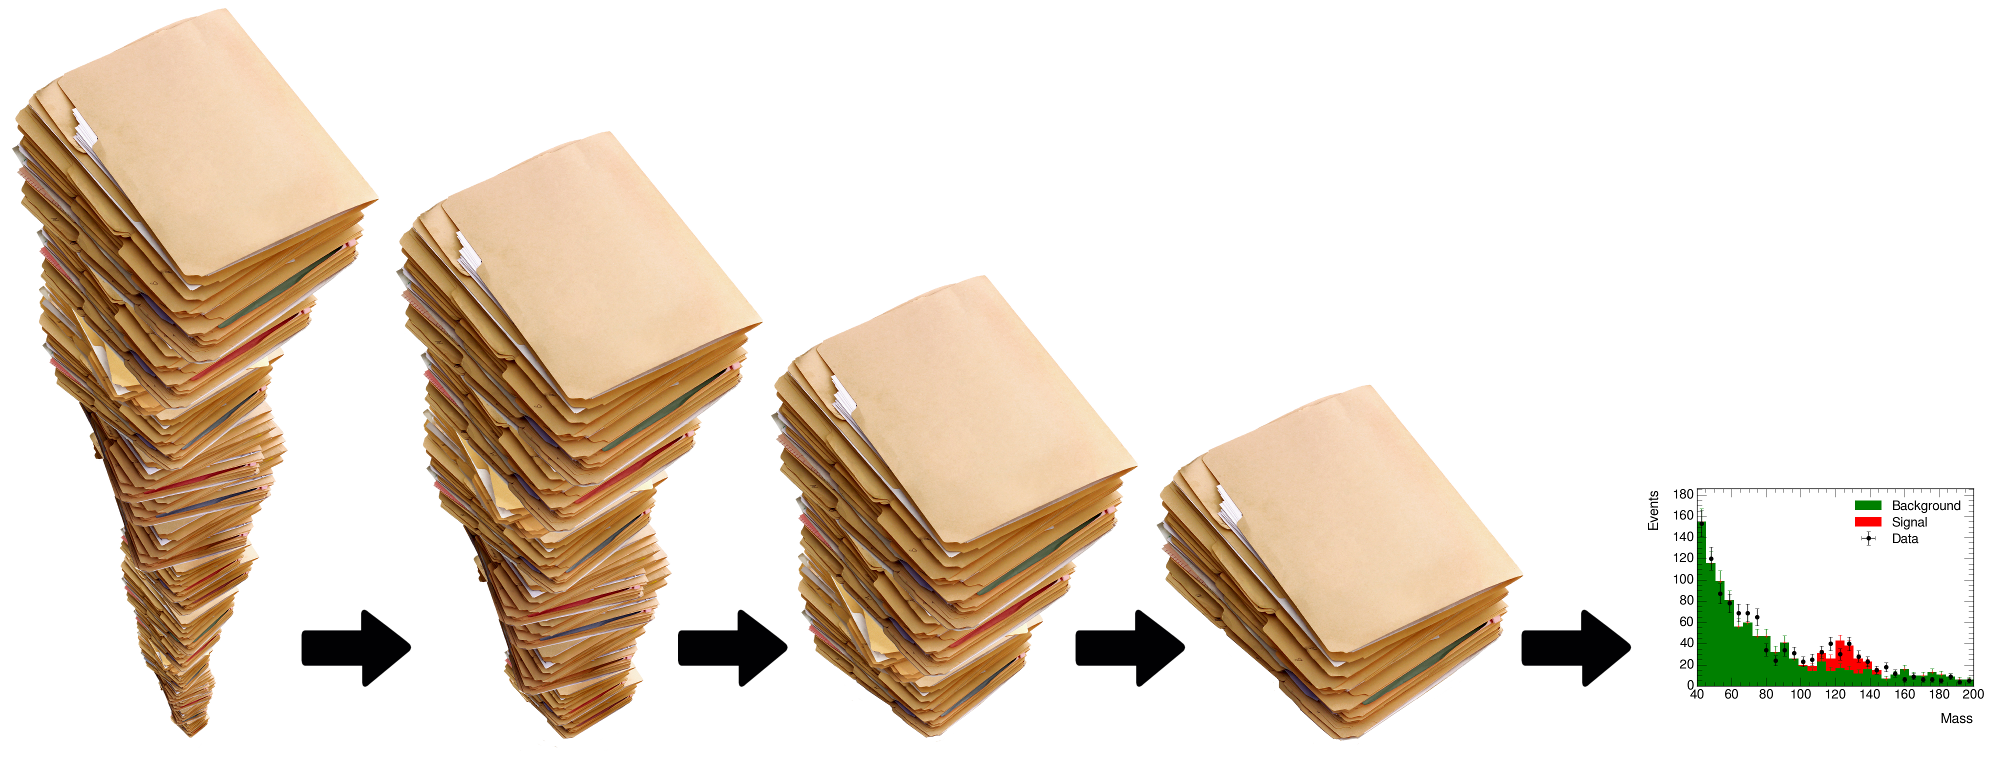
\includegraphics[width=\linewidth]{stack-of-files.png}

\vspace{0.5 cm}
Decisions about what to plot, what to cut on, and how to bin are {\it iterative} and must be close to real time.
\end{frame}

\begin{frame}{This is a problem}
Managing this chain, pushing new data through it, and keeping track of how it was made, becomes a problem in itself that distracts from the real problem of analyzing data.

\vfill
\begin{uncoverenv}<2->
\begin{center}
\begin{minipage}{0.77\linewidth}
\textcolor{darkblue}{Assertion:} if physicists could make plots (and other aggregations for statistical analysis) directly from the collaboration's Analysis Object Data in real time, they would.
\end{minipage}
\end{center}
\end{uncoverenv}
\end{frame}

\begin{frame}{Database-style interaction}
\vspace{0.5 cm}
\textcolor{darkblue}{Rapid queries on big data are possible, in fact, it's a big field:}

\vspace{0.5 cm}
\mbox{\hspace{-1 cm}

\includegraphics[height=1.23 cm]{sparksql-logo.png}

\includegraphics[height=1.23 cm]{impala-logo.png}

\includegraphics[height=1.23 cm]{ibis-logo.png}

\includegraphics[height=1.23 cm]{kudu-logo.png}

\includegraphics[height=1.23 cm]{hawk-logo.png}

\includegraphics[height=1.23 cm]{drill-logo.png}

\includegraphics[height=1.23 cm]{dremel-logo.png}

\includegraphics[height=1.23 cm]{bigquery-logo.png}}

\vspace{0.5 cm}
\begin{itemize}
\item<2-> Instead of users maintaining private resources, they share a distributed query serer.
\item<3-> Instead of fetching data from disk, \mbox{cache in RAM/SSD/X-Point.\hspace{-1 cm}}

\begin{uncoverenv}<4->
Input data required by different users has a large overlap.

Gain large factors in usable cache from {\it sharing:}

\vspace{-0.15 cm}
\[ \frac{\mbox{cache useful to each user}}{\mbox{total cache / \#users}} \gg 1 \]
\end{uncoverenv}

\item<5-> Instead of evaluating user's code as-is, transform it to optimize memory bandwidth.
\end{itemize}
\end{frame}

\end{document}
